\documentclass{report}


\usepackage{circuitikz} %Für die Schaltpläne
\usepackage[T1]{fontenc}
\usepackage[utf8]{inputenc}
\usepackage{amsmath}
\usepackage{amssymb}
\usepackage{fancyhdr}
\usepackage{graphicx}
\usepackage{hyperref}
\usepackage{subcaption}
\usepackage{tikz}
\usepackage{cite}
\usepackage[nottoc, numbib]{tocbibind}
\usepackage{../assets/scripts/tex/color-env}
\usepackage[ngerman]{babel}
\usepackage{listings}
%\usepackage{minted}

\usetikzlibrary{shapes}
    \usetikzlibrary{arrows}
    \usetikzlibrary{arrows.meta,topaths}
    \usetikzlibrary{bending}
    \usetikzlibrary{calc}
\title{Hausarbeit DI}


\usepackage[
  includehead,
  headheight = 17mm,
  footskip = \dimexpr\headsep+\ht\strutbox\relax,
  tmargin = 0mm,
  bmargin = \dimexpr17mm+2\ht\strutbox\relax,
]{geometry}

\usepackage{anyfontsize}

\usepackage{xcolor}

\definecolor{DarkGreenBlue}{HTML}{264653}
\definecolor{LightGreenBlue}{HTML}{2A9D8F}
\definecolor{LightOrange}{HTML}{E9C46A}
\definecolor{DarkOrange}{HTML}{F4A261}
\definecolor{RedOrange}{HTML}{E76F51}
\definecolor{BrightRed}{HTML}{D62828}
\definecolor{DeepBlue}{HTML}{003049}

\newcommand\invisiblesection[1]{%
  \refstepcounter{section}%
  \addcontentsline{toc}{section}{\protect\numberline{\thesection}#1}%
  \sectionmark{#1}}



\pagestyle{fancy}
\fancyhead[L]{\leftmark}
\fancyhead[R]{}
\fancyfoot[L]{}
\fancyfoot[C]{\thepage}
\fancyfoot[R]{\includegraphics[scale=0.2]{../assets/images/haw.jpg}}
\renewcommand\headrulewidth{0.5pt}


\begin{document}


\thispagestyle{empty}
\begin{tikzpicture}[remember picture,overlay]

  \fill[DeepBlue] (current page.south west) rectangle (current page.north east);

  \begin{scope}

    \foreach \i in {2.5,...,22}
      {
        \node[rounded corners, DeepBlue!90,draw ,regular polygon, regular polygon sides=6, minimum size=\i cm, ultra thick] at ($(current page.west)+(2.5,-5)$) {} ;
      }

  \end{scope}

  \node[rounded corners,fill=DeepBlue!95,text =DeepBlue!5,regular polygon,regular polygon sides=6, minimum size=2.5 cm,inner sep=0,ultra thick] at ($(current page.west)+(2.5,-5)$) {\LARGE \bfseries 2020};

  \foreach \i in {0.5,...,22}
    {
      \node[rounded corners,DeepBlue!90,draw,regular polygon,regular polygon sides=6, minimum size=\i cm,ultra thick] at ($(current page.north west)+(2.5,0)$) {} ;
    }

  \foreach \i in {0.5,...,22}
    {
      \node[rounded corners,DeepBlue!98,draw,regular polygon,regular polygon sides=6, minimum size=\i cm,ultra thick] at ($(current page.north east)+(0,-9.5)$) {} ;
    }

  \foreach \i in {12}
    {
      \node[fill = DeepBlue,rounded corners,draw=DeepBlue,regular polygon,regular polygon sides=6, minimum size=\i cm,ultra thick] at ($(current page.south east)+(-0.2,-0.45)$) {} ;
    }


  \foreach \i in {21,...,6}
    {
      \node[DeepBlue!95,rounded corners,draw,regular polygon,regular polygon sides=6, minimum size=\i cm,ultra thick] at ($(current page.south east)+(-0.2,-0.45)$) {} ;
    }

  \node[left,DeepBlue!5,minimum width=0.625*\paperwidth,minimum height=3cm, rounded corners] at ($(current page.north east)+(0,-9.5)$){{\fontsize{25}{30} \selectfont \bfseries DI - Hausarbeit}};

  \node[left,DeepBlue!10,minimum width=0.625*\paperwidth,minimum height=2cm, rounded corners] at ($(current page.north east)+(0,-11)$){{\huge \textit{Fehlersichere Übertragung und Speicherung}}};

  \node[left,DeepBlue!5,minimum width=0.625*\paperwidth,minimum height=2cm, rounded corners] at ($(current page.north east)+(0,-13)$){{\Large \textsc{Eric Antosch}}};

\end{tikzpicture}

\newpage


\tableofcontents

\listoffigures

\newpage
\renewcommand{\thechapter}{A}

\chapter{Plausibilitätsprüfung}
\label{cha:teil-plausibilitat}

\section{Einleitung}
\label{sec:einleitung}

\begin{task}
  TIn dem ersten Teilbereich der Hausarbeit soll das von einem externen Sensor erfasste 10 Bit breite Datenpacket auf hinreichende Abtastung mittels einer Plausibilitätsprüfung überprüft werden. Dabei soll das Signal $G_X$ überprüft und dann mit einem Signal $G_{XOK}$ dargestellt werden, dass das Signal zur Weiterverarbeitung übertragen werden kann.
\end{task}

Wir wollen uns zuerst einmal anschauen, was der Gray-Code überhaupt ist, um eine Idee dafür zu bekommen, mit welchen Methoden die Aufgabe bewältigen können. Während bei dem in der Digitaltechnik sehr verbreitetem Binärcode die sogenannte Hamming-Distanz unterschiedlich groß sein kann, ist der Gray-Code so konzipiert, dass diese immer nur genau 1 beträgt. Die Hamming-Distanz beschreibt dabei die Distanz zwischen zwei aufeinanderfolgenden Zahlenwerten charakterisiert als die Differenz in den Ziffern der beiden Zahlen. Die Zahl $n = 3$ und zu der Zahl $n = 4$ haben die binären Darstellungen $n_{B} = 11_{(2)}$ und $n_{B}+1 = 100_{(2)}$. Die Hamming-Distanz ist hier also $3$, da sich drei Stellen der Zahl zu der nächsten ändern. Für die Messung von Messstrecken findet sich so keine einfache Methode, die Richtigkeit bzw. Plausibilität der Werte zu testen. Im Gegensatz dazu findet sich $n_{G} = 010_{(2G)}$ und $n_{G}+1 = 110_{(2G)}$ mit einer Hamming-Distanz von $1$. Hier können wir einfach überprüfen, ob der Wert, der als nächstes eingelesen wird, sich in der Hamming-Distanz um $1$ von dem vorherigen verändert hat. Wenn nicht, so stimmt die Messung nicht vollständig oder die Auflösung ist nicht hoch genug. Besonders bei Messungen von Werten, die keine allzu starken Schwankungen erlauben, ist diese Art der Plausibilitätsprüfung sehr sinnvoll.
\newpage
\section{Blockschaltbild}
\label{sec:blockschaltbild}

Wir wollen nun zunächst das Blockschaltbild für unser Vorhaben erstellen, sodass wir bei Beschreibung des Systems in VHDL einen besseren Überblick über alle Signale und Komponenten haben.

\begin{figure}[h]
  \centering
  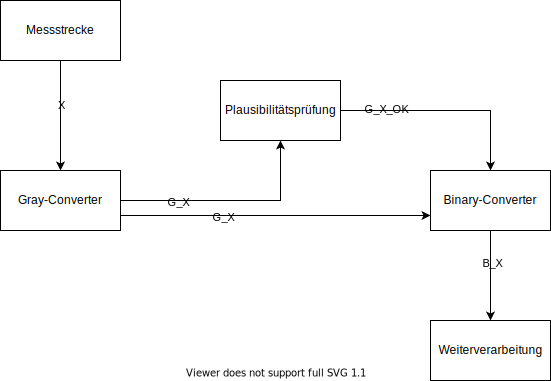
\includegraphics[width=\textwidth]{../assets/images/DIHA/blockschaltbilda.png}
  \caption{Blockschaltbild der Aufgabe A zur Plausibilitätsprüfung}
  \label{fig:blockA}
\end{figure}

\section{Lösungsidee}
\label{sec:losungsidee}

Wie schon im Einleitungstext erwähnt, bietet es sich bei dir Aufgabe an, mithilfe der Eigenschaften des Gray-Codes eine Überprüfung der Plausibilität durchzuführen. Dafür wollen nehmen wir unser Eingangssignal $G_{X}$ und speichern dies zunächst auf ein Signal buf, um es später mit dem im nächsten Zyklus eingelesenem Eingangssignal zu vergleichen. Basierend auf dem Ergebnis der Hamming-Distanz-Berechnung setzen wir $G_{XOK}$ also entweder auf True oder False. Das eingelesene Signal $G_{X}$ wird das neue buf und der Prozess wiederholt sich.

\section{Beschreibung in VHDL}
\label{sec:beschreibung-vhdl}



\section{Simulation der Ergebnisse}
\label{sec:simul-der-ergebn}

Da wir unsere Schaltung in ModelSim simulieren, verwenden wir eine .do-Datei, um den Verlauf der Schaltung zu simulieren. Wir wollen dabei sowohl den Fall erproben, dass die Daten richtig sind, als auch, dass die Daten zuweit voneinander entfernt sind, um plausibel zu sein.






\section{Fazit}
\label{sec:fazit}

Wir können anhand unserer Ergebnisse einige Dinge feststellen. Zum einen ist es wirklich erstaunlich, wie die Eigenschaften von speziellen Codes die Verarbeitung und Implementierung von bestimmten Lösungen vereinfacht. Die Logik, um eine solche Plausibilitätsprüfung durchzuführen, wenn die Eingangsdaten zum Beispiel weiterhin als Binärcode kodiert sind, wäre um einiges komplizierter und außerdem nicht wirklich effizient oder wirtschaftlich. Es bietet sich also stark an, die Möglichkeit von den verschiedenen Codes aus der Digitaltechnik einzustudieren. Es ist außerdem ersichtlich, dass sich eine Darstellung von Problemstellungen nach dem gelernten Schema anbietet. Es lässt einen stark über die einzelnen Komponenten und die Zusammenarbeit auf einem tatsächlichen FPGA-Board nachdenken.


\renewcommand{\thechapter}{B}

\chapter{Berechnung der Regelabweichung}
\label{cha:berechn-der-regel}

\section{Einleitung}
\label{sec:einleitung-1}

\begin{task}
  TIn der nächsten Aufgabe soll es um die Berechnung der Regelabweichung von zwei Signalen mithilfe eines Carry-Lookahead-Addierers gehen. Dabei ist unser auf Plausibilität geprüfte Signal $B_X$ mit einem Sollwert $B_{W}$ zu vergleichen und die Differenz auf einer bidirektionalen 10-bit breiten Busleitung auszugeben. Ebenfalls sollen die dedizierten Signale EXAKT und ZU\_KLEIN seperat je nach Ergebnis ausgegeben werden.

\end{task}


\section{Blockschaltbild}
\label{sec:blockschaltbild-1}

\begin{figure}[h]
  \centering
  \includegraphics[width=\textwidth]{../assets/images/DIHA/delta.png}
  \caption{Blockschaltbild für die Regelabweichung}
  \label{fig:blockregel}
\end{figure}



\section{Automatengraph}
\label{sec:automatengraph}


\section{Lösungsidee}
\label{sec:losungsidee-1}

Wir wollen uns nun einmal anschauen, mit welchen Mitteln wir unser Ziel erreichen können.

\subsection{Carry-Lookahead-Addierer}
\label{sec:carry-look-addi}

Bei dem Carry-Lookahead-Addierer, den wir für unsere Berechnung der Regelabweichung verwenden wollen, handelt sich um eine Weiterentwicklung des Carry-Ripple-Addierers. Hier werden also nicht einfach nur mehrere Volladdierer miteinander so verschaltet, dass mehrere Bit breite Signale miteinander addiert werden können, sondern es gibt ein komplizierteres System, um die Übertrage der Volladdierer zu bestimmen. Fundamental für diese Überlegung sind die Konzepte von Generate, Propagate und Absorb.

\paragraph{Generate}

Bei Generate handelt sich um ein logisches Prädikat, welches wir im Folgenden durch $G(A, B)$ bezeichnen möchten mit $G(A,B) = A \cdot B$, wobei $\cdot$ das logische Und darstellt. Wir sagen also, dass zwei Ziffern genau dann generieren, wenn die beiden Ziffern immer einen Übertrag bilden und dieser nicht abhängig ist, ob ein weiterer Übertrag auf die Ziffern hinzuaddiert werden.

\paragraph{Propagate}

Bei Propagate handelt es sich ebenfalls um ein logisches Prädikat, welches wir im Folgenden mit $P(A,B) = A + B$ bezeichnen, wobei $+$ das logische Oder darstellt. Wir sagen also, dass zwei Ziffern genau dann propagieren, wenn die beiden Ziffern nur dann einen Übertrag bilden, wenn ein weiterer Übertrag von der Berechnung vorher kommt.

\paragraph{Absorb}

Wir wollen im folgenden Absorb als denjenigen Zustand definieren, der einen Übertrag von der vorherigen Berechnung absorbieren würde, dabei allerdings keinen Übertrag generiert. Mit $A(A,B) = \not(A + B)$ definieren wir einen Zustand, der das Gegenteil von Propagate darstellt und nur dann wahr ist, wenn beide Ziffern (im Falle einer binären Addition) $0$ sind.

\subsection{Zweier Komplement}
\label{sec:zweier-komplement}

Wenn wir die Differenz von zwei binären Zahlen berechnen wollen, müssen wir eine der beiden, da unser Carry-Lookahead-Addierer eigentlich nur Addition beherrscht, in ein anderes Format umwandeln, um eine Differenz berechnen zu können. Wir entscheiden uns hier für das Zweier Komplement, um aus einer der beiden Signalen, die eine binäre Zahl darstellen, eine negative Zahl zu machen, und diese dann zu addieren.

Bei der Umwandlung gehen wir dabei nach folgendem Schema vor:

\begin{enumerate}
  \item Das Most-Significant-Bit stellt im zweier Komplement das Vorzeichen dar, wir setzen dies also auf eine $1$, um ein Minus-Zeichen darzustellen
  \item Wir invertieren alle weiteren Bits, alle $1$ werden zu $0$ und umgekehrt.
  \item Zum Schluss addieren wir auf die Zahl eine $1$, unsere Zahl ist damit umgewandelt.
\end{enumerate}

\subsection{Taktsynchronität}
\label{sec:taktsynchronitat}

Wir müssen uns nun noch mit der Anforderung an unsere Lösung beschäftigen, taktsynchron und in Harmonie mit dem Busarbiter zu funktionieren. Dafür wollen wir in unserer Beschreibung mit VHDL eine eigene Komponente einrichten, die sich um genau diese Anforderungen kümmert.

\section{Beschreibung in VHDL}
\label{sec:beschreibung-vhdl-1}

\section{Simulation der Ergebnisse}
\label{sec:simul-der-ergebn-1}

\section{Fazit}
\label{sec:fazit-1}



\end{document}
%%% Local Variables:
%%% LaTeX-command: "latex -shell-escape"
%%% End:
